\documentclass{beamer} 
\usetheme{default} 
\usecolortheme{albatross}
\setbeamercovered{transparent}
%\useoutertheme{umbcfootline}  


\usepackage[spanish]{babel}
%\usepackage[latin1]{inputenc}
\usepackage[utf8x]{inputenc}
\usepackage{hyperref}
\usepackage{color}
\usepackage{multicol}
%%codigo java

 

%\usepackage[usenames,dvipsnames]{color}
\title{Clase genérica, colecciones y comparadores}

\author{Manuel J. Molino Milla \and Luis Molina Garzón}

\date{\today} %

\institute{IES Virgen del Carmen \and Departamento de Informática}




%\beamerdefaultoverlayspecification{<+->}

\begin{document}


\begin{frame}
  \titlepage
\end{frame}

\begin{frame}
    \frametitle{Logo}
\begin{figure}

\includegraphics[scale=1]{imagenes/logo.jpeg} 
\caption{Logo Java}
\end{figure}
\end{frame}

%\begin{frame}
 % \frametitle{Contenido}
 %\tableofcontents[pausesections]
%\end{frame}



%\section{Framework Collection}

%\begin{frame}
%\frametitle{Colecciones en java}
%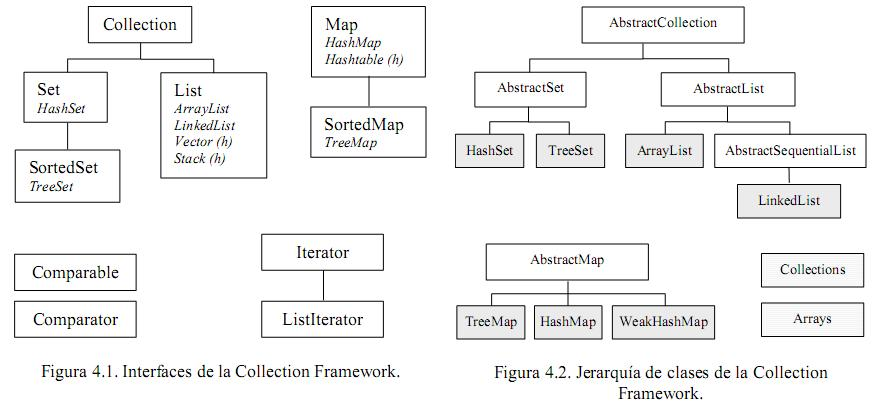
\includegraphics[scale=0.45]{imagenes/colecciones.jpeg}
%\end{frame}

\section{Genéricos} 
\begin{frame}[fragile]
\frametitle{Clases genéricas}
\emph{Son clases cuyos atributos son genéricos (Object)
}
\begin{verbatim}
public class Generico {
  private Object atributo;
  
  public void setAtributo (Object atributo){
    this.atributo = atributo;  
  }
  
  public Object getAtributo(){
    return atributo;
  }
}
\end{verbatim}
\pause
\emph{En un main de una clase:}
\begin{verbatim}
Generico generico = new Generico();
generico.setAtributo("atributo");
String atributo = (String) generico.getAtributo();
\end{verbatim}

\end{frame}

\begin{frame}[fragile]
\frametitle{Clases parametrizadas}
\emph{A partir de Java 5 se permite clases parametrizadas}
\begin{verbatim}
public class Parametrizado<T> {
  private T atributo;
  
  public void setAtributo (T atributo){
    this.atributo = atributo;  
  }
  
  public T getAtributo(){
    return atributo;
  }
}
En un main de una clase haríamos:

Generico<String> generico = new Generico<>();
generico.setAtributo("atributo");
String atributo = generico.getAtributo();
\end{verbatim}
\end{frame}


\begin{frame}[fragile]
\frametitle{Clases parametrizadas con dos tipos}
\begin{verbatim}
public class Parametrizado<T, S> {

  private T atributoT;
  private S atributoS;
  
  .................

}
\end{verbatim}
\end{frame}


\begin{frame}
\frametitle{Convencciones para nombrar genéricos}
\begin{description}[<+->]
\item[T] Type (Representa un tipo, es decir, una clase)
\item[E] Element (usado bastante por Java Collections Framework)
\item[N] Number (para números)
\item[V] Value (representa el valor, también se usa en diccionarios)
\item[S,U,V ...] Para tipos
\end{description}

\end{frame}

\begin{frame}[fragile]
\frametitle{Genéricos con tipos}
Podemos indicar el tipo del genérico
\begin{verbatim}
public class Parametrizado<T extends Number> {

  private T atributoT;
 
  .................

}
\end{verbatim}
¿Qué tipos permite la clase Number?
\end{frame}

\begin{frame}[fragile]
\frametitle{Tipos comodin}
\begin{itemize}[<+->]
\item Muy útil con colecciones. 
\item Nos permite relajar el tipo
\end{itemize}
\pause
\begin{verbatim}
public static double sumaLista(
         List<? extends Number> lista) {
  double suma = 0.0;
  for (Number numero : lista){
    suma += numero;
  }
  return suma;
}
\end{verbatim}
\end{frame}


\section{Colecciones}

\begin{frame}
\frametitle{API COLLECTIONS}
\begin{figure}
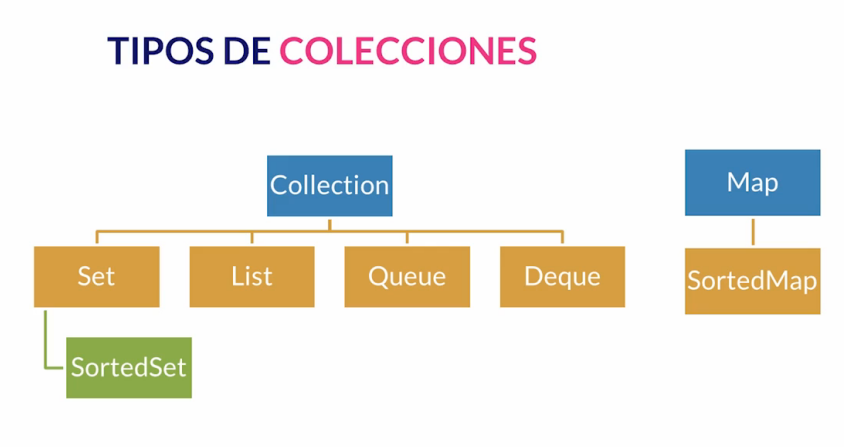
\includegraphics[scale=0.5]{imagenes/colecciones1.png}
\end{figure}
\end{frame}

\begin{frame}
\frametitle{TIPO DE COLECCIONES}
\begin{figure}
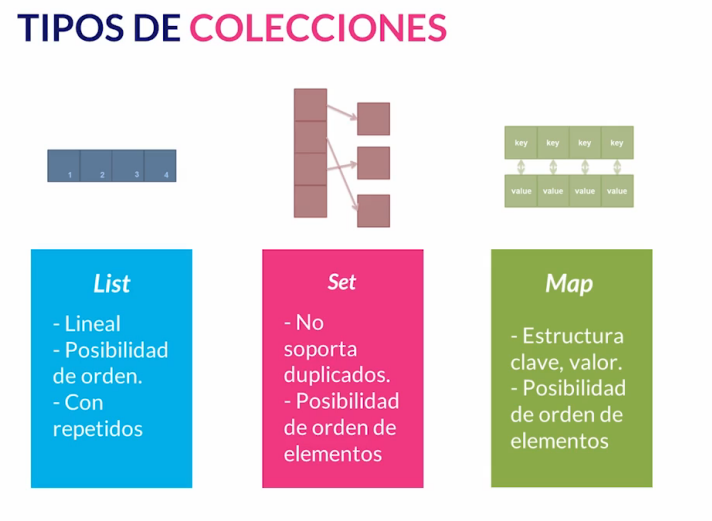
\includegraphics[scale=0.5]{imagenes/colecciones2.png}
\end{figure}
\end{frame}


\begin{frame}[fragile]
\frametitle{Interfaz List}
\begin{itemize}[<+->]
\item Permite objetos duplicados.
\item Las mas usadas son \emph{ArrayList} y \emph{LinkedList}
\item Generalmente usaremos la primera.
\item Una clase mas antigua y parecida es la clase \emph{Vector}
\item Funciona igual que \emph{ArrayList}
\end{itemize}
\pause
\begin{block}{Ejemplo de uso}
\begin{verbatim}
List<Persona> listaPersonas = new ArrayList<>();
\end{verbatim}
\end{block}
\end{frame}



\begin{frame}
\frametitle{Metodos de List}
\begin{description}
\item[add] Añade un elemento al final de la lista.
\item[addAll] Añade los elementos de una colección a la lista.
\item[clear] Elimina todos los elementos de la lista.
\item[contains] Nos dice un si un elemento está en una lista.
\item[get] Nos devuelve un elemento de la lista.
\item[isEmpty] Nos dice si la lista que está vacía.
\item[remove] Elimina un elemento de la lista.
\item[size] Nos dice el tamaño de la lista.
\item[toArray] Convierte la lista en un array.
\end{description}
\end{frame}

\begin{frame}[fragile]
\frametitle{Interfaz Set}
\begin{itemize}[<+->]
\item No permite objetos duplicados.
\item Propone tres subtipos:
\begin{description}
\item[HashSet] es la mas eficiente, pero no asegura el orden.
\item[TreeSet] asegura un orden, eficiente en búsqueda pero no en inserción.
\item[LinkedHashSet] igual que \emph{HashSet} pero mantiene orden.
\end{description}
\end{itemize}
\pause
\begin{block}{Ejemplo de uso}
\begin{verbatim}
Set<Persona> listaPersonas = new HashSet<>();
\end{verbatim}
\end{block}
\end{frame}

\begin{frame}
\frametitle{Metodos de Set}
Idénticos a los de \emph{List}
\begin{description}
\item[add] Añade un elemento al final de la lista.
\item[addAll] Añade los elementos de una colección a la lista.
\item[clear] Elimina todos los elementos de la lista.
\item[contains] Nos dice un si un elemento está en una lista.
\item[get] Nos devuelve un elemento de la lista.
\item[isEmpty] Nos dice si la lista que está vacía.
\item[remove] Elimina un elemento de la lista.
\item[size] Nos dice el tamaño de la lista.
\item[toArray] Convierte la lista en un array.
\end{description}
\end{frame}


\begin{frame}[fragile]
\frametitle{Interfaz Map}
\begin{itemize}[<+->]
\item No es clase hija de \emph{Collections} como lo son \emph{List} y \emph{Set}
\item Propone tres subtipos: \emph{HashMap, TreeMap y LindkedHashMap} de características
\item Cada elemento tiene una estructura clave/valor
\item Se le conoce como diccionarios.
\item La clave nos sirve para obtener el valor (como los diccionarios) 
\end{itemize}
\pause
\begin{block}{Ejemplo de uso}
\begin{verbatim}
Map<Integer, String> map = 
                     new HashMap<Integer, String>();
\end{verbatim}
\end{block}
\end{frame}


\begin{frame}
\frametitle{Métdos Map}
\begin{description}
\item[put] Inserta un par clave/valor.
\item[containsKey] Comprueba si una clave está en un \emph{Map}
\item[containsValue] Comprueba si un valor está en un \emph{Map}
\item[clear] Elimina todos los elementos del \emph{Map}.
\item[get] Nos devuelve el valor de una clave.
\item[isEmpty] Nos dice si el \emph{Map} está vacío.
\item[remove] Elimina un elemento del \emph{Map}.
\item[size] Nos dice el tamaño del Map.
\item[values] Nos devuelve un \emph{Collection} de los valores
\item[keySet] Nos devuelve un \emph{Set} de las claves
\end{description}
\end{frame}


\begin{frame}
\frametitle{Comparando Objetos}
\begin{itemize}[<+->]
\item A veces hay que comparar objetos. 
\item En el caso de los tipos primitivos existe un orden, en el caso de los números un orden natural, en tipo \emph{char} el orden lexicográfico.
\item Es muy normal tener que implementar ese orden en las clase básicas.
\end{itemize}
\end{frame}

\begin{frame}[fragile]
\frametitle{Interfaz Comparable}
\begin{verbatim}
public Interface Comparable<T> {
  public int compareTo(T o);
}
\end{verbatim}
\pause
\begin{itemize}[<+->]
\item Se trata de comparar objetos del mismo tipo.
\item Devuelve \textbf{0} si son iguales.
\item Un valor \textbf{negativo} si es menor.
\item Un valor \textbf{positivo} si es mayor.
\end{itemize}
\end{frame}

\begin{frame}[fragile]
\frametitle{Interfaz Comparator}
\begin{verbatim}
public Interface Comparator<T> {
  public int compare(T o1, T o2);
}
\end{verbatim}
\pause
\begin{itemize}[<+->]
\item Ahora el método recibe los dos objetos.
\item Devuelve \textbf{0} si son iguales.
\item Un valor \textbf{negativo} si es menor.
\item Un valor \textbf{positivo} si es mayor.
\item Ha diferencia del anterior no se hace sobre la clase básica, sino cuando hace falta en un momento dado hacer una comparación.
\end{itemize}
\end{frame}
\end{document}